%!TEX root = ../../main.tex

\section{Evaluation Protocol} \label{sec:protocol}
    The leave-one-actor out cross validation strategy represented in \cite{Stone1974} is employed and average accuracy (\%) are computed as means of comparison.
    In order to evaluate the proposed framework in terms of cross-view performance, it is further combined with cross-view validation.
    That means at a moment only two views are picked to evaluate, each consists of a train and a test part defined by the leave-one-actor out strategy.
    Apart from the proposed evaluation protocol, from now named ``\emph{protocol 1}'', another ``\emph{protocol 2}'' is assessed, which is regularly used in the literature.
    The main difference is in second protocol, the notation of train or test is omitted after feature extraction stage, every features samples from single view are included to train the multi-view metrics, then the classifier is fit on common features of one view and tested on common features of another view.
    It is noticed that the first evaluation protocol is more challenging because the in the second protocol, the constructed common space is already fit on the whole multi-view dataset. As a result, the later predictive models are trained and evaluated on features generated by a severely over-fitted projector. % Details about two evaluation protocols is presented in supplemental materials. 
    The difference between two protocols are illustrated in Figure \ref{Fig:ep}. 

    \begin{figure}[htbp]
      \centering
      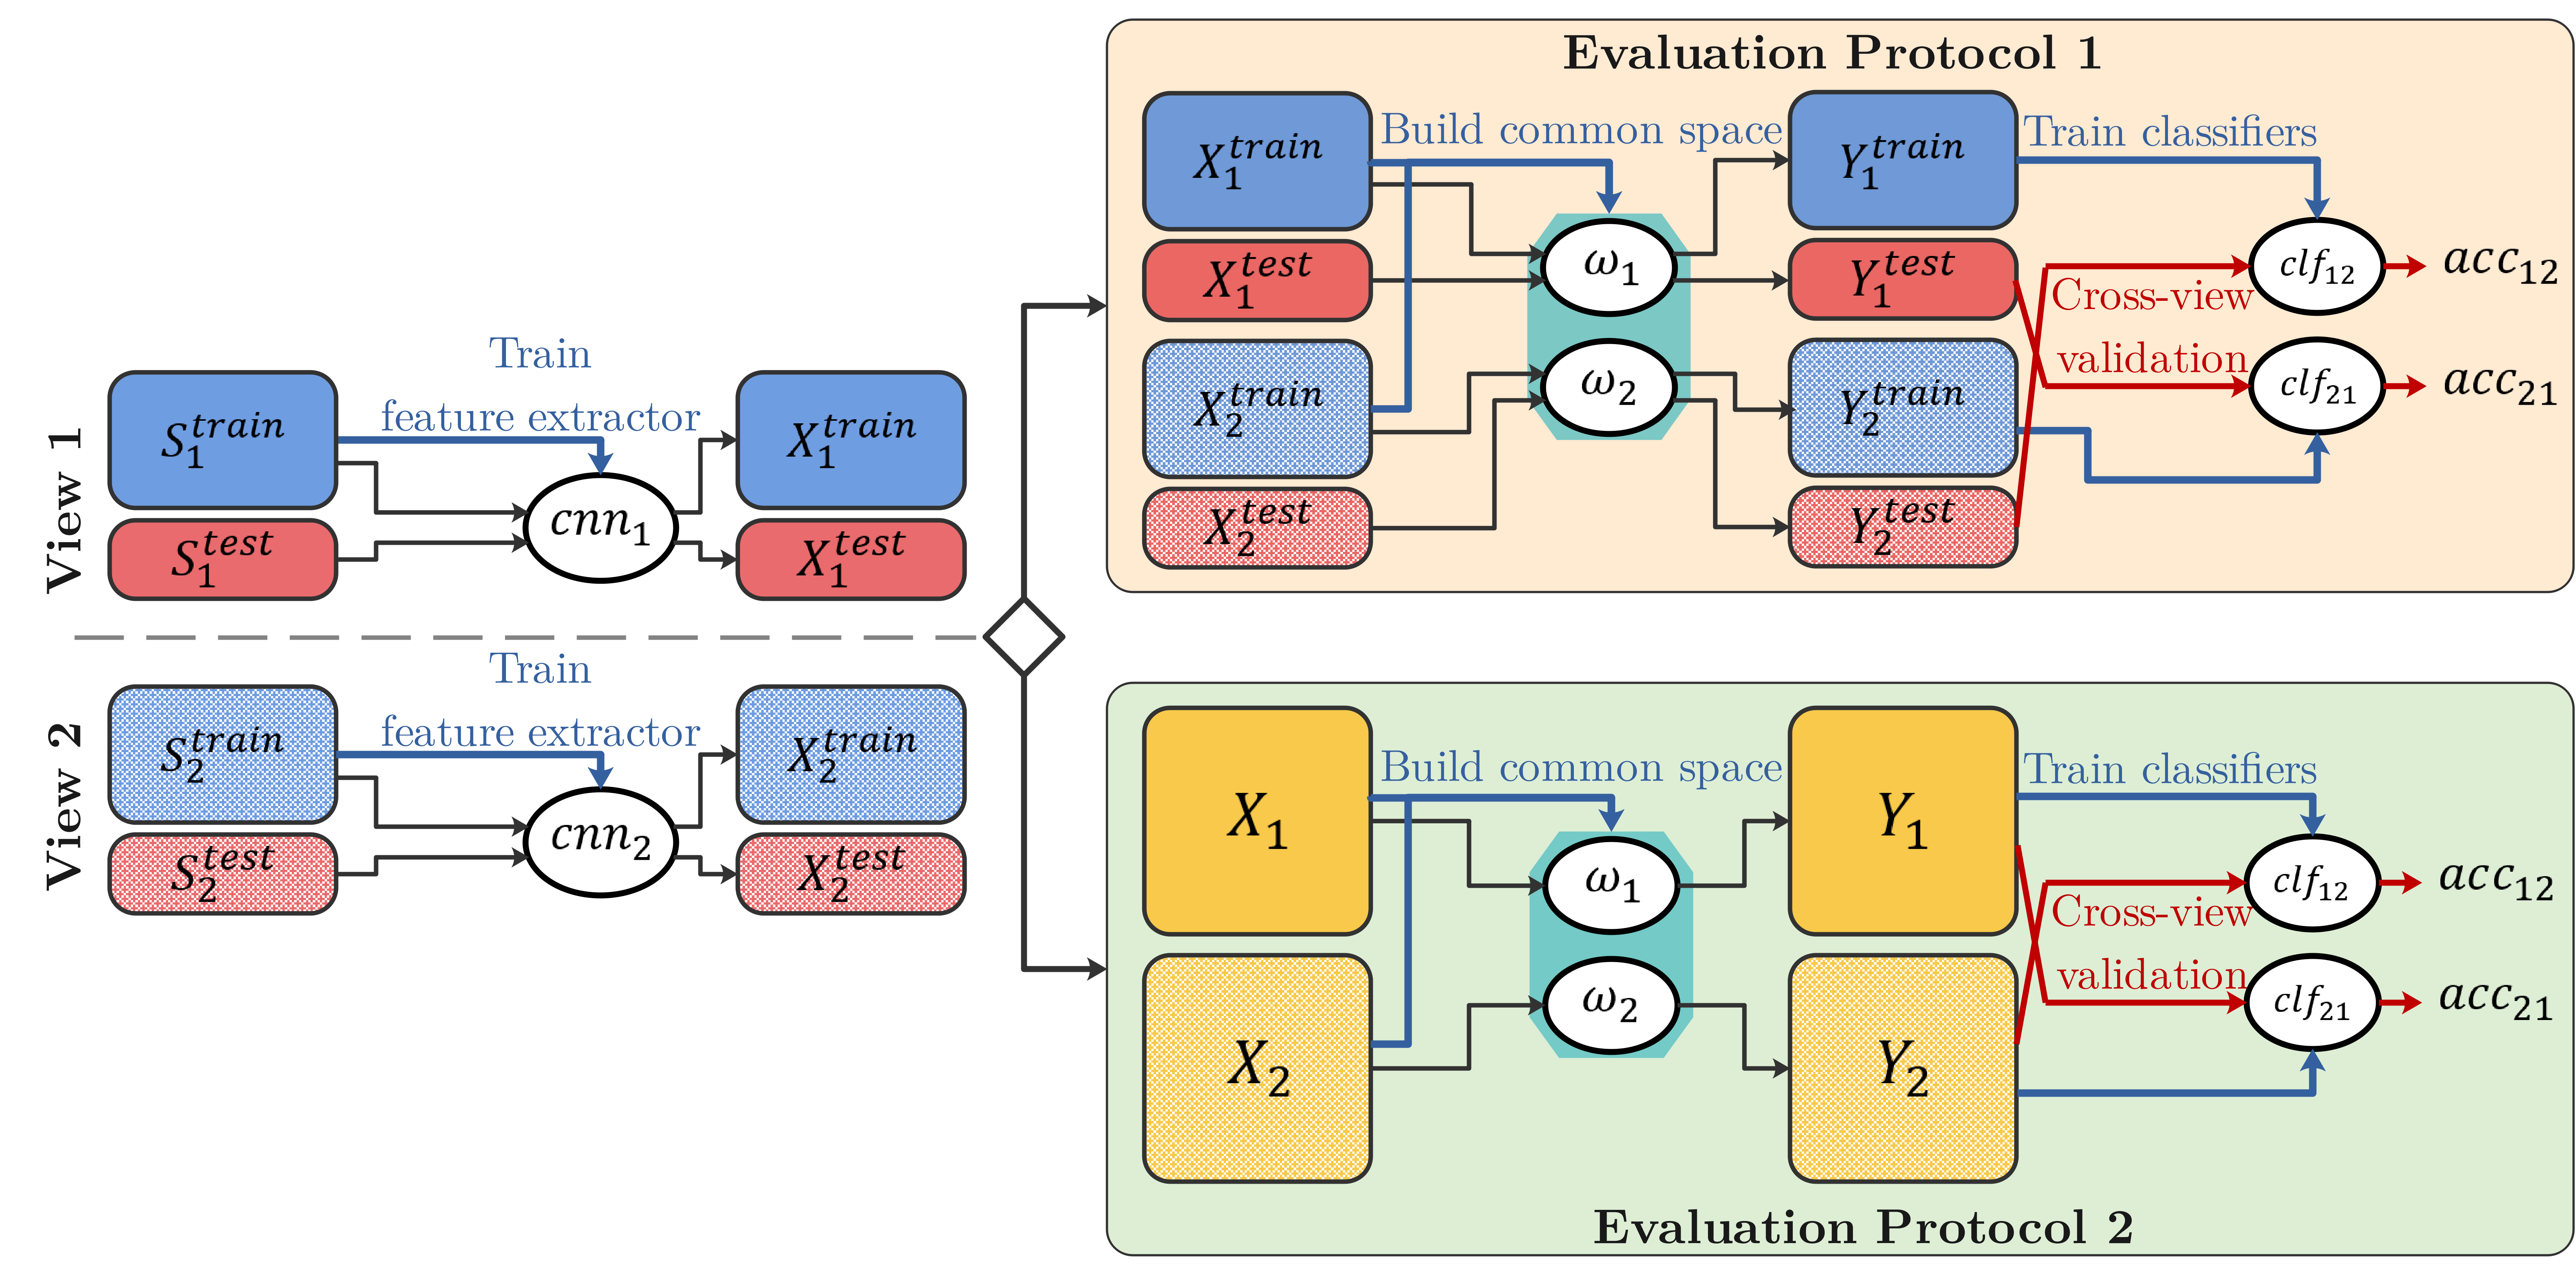
\includegraphics[width=1\linewidth]{figs/protocol.png}
      \caption{Two evaluation protocols used in experiments.}
        %\vspace{-0.3cm}
      \label{Fig:ep}
    \end{figure}
    The overall cross-view evaluation score is computed as average of all evaluation scores of each split, whose method of computation is described specifically in Figure \ref{Fig:ep}:
    \begin{equation}
        {acc}_{ij} = \frac{\sum_{k=1}^M {acc}^{(k)}_{ij}}{M}
    \end{equation}
    where M is the number of actors. Both protocols finally generate a cross-view accuracy matrix as follows:
    \begin{equation}
        \left[\begin{matrix}{acc}_{11}&{acc}_{12}&\cdots&{acc}_{1v}\\{acc}_{21}&{acc}_{22}&\cdots&{acc}_{2v}\\\vdots&\vdots&\ddots&\vdots\\{acc}_{v1}&{acc}_{v2}&\cdots&{acc}_{vv}\\\end{matrix}\right]
        \label{eq:multi-view_scores}
    \end{equation}
    For eager expression, let's define function $\operatorname{accuracy}\left(Y, \tilde{Y}\right)$ as the accuracy score when fitting a classifier on $Y$ features and evaluating its prediction on $\tilde{Y}$ features. Each cell can be expressed accordingly:
    \begin{align}
        {score}_{jr}^{\boldsymbol{protocol 1}} & =\left<\left\{\operatorname{accuracy}\left(Y_j^{train},Y_r^{test}\right)\middle|\ j,r=(1,..,v)\right\}\right> \\
        {score}_{jr}^{\boldsymbol{protocol 2}} & =\left<\left\{\operatorname{accuracy}\left(Y_j,Y_r\right)\middle|\ j,r=(1,..,v)\right\}\right>
    \end{align}

    \textbf{Multi-view strategy:} As MvDA and its variants can theoretically scale for an arbitrary number of views, in order to fairly compare the proposed algorithm with others that only apply for 2 views, we also experiment 2 different multi-view strategies. The key idea is that each strategy restricts the number of views participated in the training process of MvA algorithms.

    In ``\emph{multi-view}'' strategy, only one set of $W^*=\left\{{\omega}_1, {\omega}_2, ..., {\omega}_v\right\}$ is learnt and all separated view features are transformed $Y_j=\omega_j^TX_j,\ j=(1,...,v)$ before computation of accuracy.

    In ``\emph{cross-view}'' strategy, each cell ${score}_{jr}$ of \eqref{eq:multi-view_scores} must be calculated exclusively with the inclusion of only features of those views $j$ and $r$ (wihtout information from other views).
    Therefore, for each distinct combination $jk$, $W_{jr}^*=\left\{{\omega}_j, {\omega}_r\right\}$ is learnt to transform $X_j$ and $X_r$. The diagonal of \eqref{eq:multi-view_scores} is also ignored in this strategy.

    Since there are many scores generated by such extra complicated cross validation process when cycling through every actors, the final reported is average of all.
    Further, it is noticed that in existing works, the evaluation have been done mostly similar to the second evaluation protocol. Hence, in comparison with state of the art techniques, only the scores resulted from the second evaluation protocol are taken.
